The watch prototype is severely limited in its ability to deliver a high throughput and low latency video stream to the edge, hindering the benefits of edge computing. In order to better take advantage of cloudlet resources, a new offload device is needed which can transmit the video stream without the thermal restrictions of the watch. As discussed in Section~\ref{sec:achieving-cell-conn}, there are no current Android products other than smart watches that satisfy the stringent weight requirements of the Parrot Anafi platform. The only path forward is to explore other segments of the mobile computing landscape.

In this chapter, I propose a new offload device which fixes some of the shortcomings of the watch prototype. I will show how it improves upon the watch in some ways but fails to match its capabilities in others. In Section~\ref{sec:watch-replacement}-\ref{sec:onion-omega-payload}, I explain the process of choosing a new device. I give a breakdown of its control model and how it differs from the watch. In Section~\ref{sec:ooda-intro}-\ref{sec:e2e-discussion}, I use an agility analysis framework to compare the overall performance of each prototype.

\section{Finding a Watch Replacement}
\label{sec:watch-replacement}

For any device to replace the watch, it must satisfy three main requirements of the SteelEagle pipeline: WiFi connectivity, cellular connectivity, and light weight. The first two requirements, WiFi and cellular connectivity, are relatively easy to find within the mobile device space. Meeting the weight requirement is much harder. The Parrot Anafi was able to fly with the watch payload, around 39~g, but was unable to fly with the Unihertz Jelly Pro payload, around 90~g with EMI shielding included. This gives an approximate weight range for a watch replacement.

Outside of smart watches, the only devices that lie within this weight range are single-board computers (SBCs). SBCs are small form factor computers which live on a board about the size of a credit card. They are widely used for internet of things (IoT) projects because of their small size, low power draw, and connectivity (usually WiFi but sometimes cellular as well). The most popular SBC at the time of writing this dissertation is the Raspberry Pi~\cite{RaspberryPi}. The Pi is an Ubuntu SBC available in several sizes, the lightest of which is the Pi Zero 2 W at 16~g (Figure~\ref{fig:pi-zero}). The Zero is equipped with a quad-core 1~GHz CPU and 512~MB of RAM. It has built-in WiFi connectivity but must be augmented with a dongle for cellular connectivity. Additionally, it does not come with an integrated battery, so it must be powered by an external power pack that provides 1.2~A at 5.5~V. I determined that EMI shielding was not needed since the Pi did not create enough interference to hinder the Anafi's compass. With a power pack, 4G LTE dongle, and mount included, a Pi Zero payload for the Anafi would reach around 80~g. From experimentation, I found this was too heavy as the drone exhibited poor flight characteristics. A lighter alternative was needed.

\begin{figure}
    \centering
    \includegraphics[width=0.4\linewidth]{chapter5/FIGS/zero2.png}
    \begin{captext}
    \small \\[0.1cm] The Pi Zero 2 W is 16~g but lacks cellular connectivity and requires an external power source. 
    \end{captext}
    \caption{Raspberry Pi Zero 2 W~\cite{RaspberryPi}}
    \label{fig:pi-zero}
\end{figure}

\begin{figure}
    \centering
    \vspace{-0.5in}
    \includegraphics[width=0.4\linewidth]{chapter5/FIGS/onion.png}
    \vspace{-0.5in}
    \begin{captext}
    \small \\[0.1cm] The Onion Omega is 20~g with embedded WiFi and 4G. It requires a 3.3~V, 0.5~A power source. 
    \end{captext}
    \caption{Onion Omega 2 LTE~\cite{Onion}}
    \label{fig:onion}
\end{figure}

After an extensive search, I settled on the 20~g Onion Omega 2 LTE (Figure~\ref{fig:onion})~\cite{Onion}. The Omega is another SBC with built-in WiFi and 4G LTE connectivity. It runs OpenWRT Linux and is equipped with a single-core 580~MHz CPU and 128~MB of RAM. This makes it much less powerful, on paper, than the Galaxy Watch 4 (1.18~GHz dual-core CPU, 1.5~GB RAM). It also does not have an integrated battery, and like the Pi, does not create enough interference to warrant EMI shielding. However, unlike the Pi, the Onion only requires 0.5~A at 3.3~V which allows it to be powered by a much smaller, lighter power pack. This means, after adding a mount, power pack, and antennas, the Onion payload is a much slimmer 53~g. Through experimentation, I found this weight to be viable for sustained flight without adverse flight effects.

\begin{figure}
    \centering
    \includegraphics[width=1.0\linewidth]{chapter5/FIGS/arch-onion.png}
    \begin{captext}
    \\[0.1cm]
        \small The Onion acts as a pure relay, ferrying low-level command packets from the drone to the cloudlet. There, they are collected by a ``drone proxy'' which acts similarly to the watch in Figure~\ref{fig:sys-arch}.
    \end{captext}
    \caption{SteelEagle System Architecture with Onion Omega}
    \label{fig:sys-arch-onion}
\end{figure}

\section{The Onion Omega Payload}
\label{sec:onion-omega-payload}

The Onion's onboard compute resources are much worse than the Galaxy Watch 4. Its advantage is its thermals; it can run much, much hotter than the watch before overheating. This is mainly because it is not designed to be worn, and thus does not need to worry about burning its wearer. As a result, the Onion can transmit over its 4G link at a high rate without restrictions.

The Onion cannot run a full-featured local application like the watch can, but its ability to use cellular connectivity without constraints suggests a different control paradigm. Rather than controlling the drone locally from the watch and only sending frames to the cloudlet to run computer vision algorithms, the Onion can act as a pure relay, ferrying telemetry and video packets upstream while delivering command packets downstream. In this system, the watch application would migrate to the cloudlet and would communicate with the drone over the Onion (Figure~\ref{fig:sys-arch-onion}). This is known as the ``thin client'' computational paradigm.

This approach has some advantages. First, it theoretically allows the cloudlet to receive the raw video stream from the drone at full frame rate and relatively low latency (compared to the watch). Since the Onion does no video decoding, the latency cost paid is simply the transmission delay from the drone to the Onion over WiFi and from the Onion to the cloudlet over 4G. Second, the mission application lives on the cloudlet and so it can get computer vision results with negligible latency.

On the other hand, this setup has significant drawbacks compared to the watch. The Onion payload is not as robust as the watch payload. It has exposed electronics and requires the use of a flammable LiPo power pack to use, whereas the watch is a consumer device that is easy to charge and is fully weatherproofed. Furthermore, since the Onion acts as a pure relay, it is at the mercy of its cellular connection. It cannot function separately from the cloudlet, while the watch can still pilot the drone without computer vision assistance. It also cannot adapt the video stream to reduced bandwidth by throttling, and must transmit the whole stream to produce usable frames on the backend.

Despite these problems, the Onion presents an opportunity to establish an upper bound for SteelEagle's performance. Where are the current bottlenecks in the system, and how can they be fixed? What is the best latency and throughput the system can achieve? How \textit{agile} is the system at reacting to new stimuli?

\section{A Framework for Understanding Agility: the \ooda~Loop}
\label{sec:ooda-intro}
To answer these questions, I introduce the concept of a drone \ooda~loop. Originally conceived in the 1950s to characterize
man-machine symbiosis in combat aircraft, this concept has
since been extended to many other domains~\cite{Boyd1986, Blaha2018, Johnson2023}.  The components of an \ooda~loop~(``Observe'', ``Orient,'' ``Decide,'' and
``Act'') define the stages of any reactive pipeline that involves a
human in the loop.  I extend this concept from its
cyber-human origins to the cyber-physical context of an autonomous
drone.  Viewing an AI pipeline through the lens of an \ooda~loop better explains its performance attributes.  It can tease apart latency and throughput limitations at fine granularity, thus enabling bottlenecks to be identified and optimized.

An \ooda~loop's attributes directly limit drone agility.  As discussed in Section~\ref{sec:event-to-detection-latency}, throughput limitations may cause closely-spaced real-world events to not be
resolvable as separate events.  High end-to-end latency
may cause slow reactions and punish mis-predictions. SteelEagle's \ooda~loop includes: (a) on-drone sensing, (b) on-drone
pre-processing, (c) transmission to cloudlet, (d) processing on a
(possibly multi-tenant) cloudlet, (e) transmission to drone, (f)
on-drone post-processing, and (g) drone actuation. I will profile and optimize these components through experimentation.

\begin{figure}
	\definecolor{observe-color}{RGB}{175,208,149}
	\definecolor{orient-color}{RGB}{255, 255, 166}
	\definecolor{decide-color}{RGB}{255,170,149}
	\definecolor{act-color}{RGB}{224,194,205}
	\centering
	\includegraphics[width=0.9\linewidth]{chapter5/FIGS/fig-ooda-loop.pdf}
	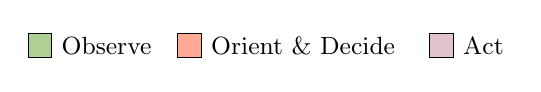
\begin{tikzpicture}
	    \draw[fill=observe-color] (1.0,0) rectangle (1.3,0.3);
	    \node[right] at (1.3,0.15) {\small Observe};
	
	    \draw[fill=decide-color] (2.9,0) rectangle (3.2,0.3);
	    \node[right] at (3.2,0.15) {\small Orient \& Decide};
	
	    \draw[fill=act-color] (6.1,0) rectangle (6.4,0.3);
	    \node[right] at (6.4,0.15) {\small Act};
	\end{tikzpicture}
	\caption{Detailed View of the \ooda~Loop}
	\label{fig:ooda-loop}
	\vspace{0.2in}
	\centering
	\includegraphics[width=0.8\linewidth]{chapter5/FIGS/fig-ooda-nomenclature.pdf}
	\begin{captext}
		\centering \\[0.1cm] Only items in \textcolor{red}{red} above can be measured.
		\flushleft
		\begin{tabular}{lll}
			\phantom{00} & a = on-drone sensing & e = transmission to drone\\
			\phantom{00} & b = on-drone pre-processing & f = on-drone post-processing\\
			\phantom{00} & c = transmission to cloudlet & g = drone actuation\\
			\phantom{00} & d = processing on cloudlet\\
		\end{tabular}
	\end{captext}
	\caption{Measurable Components of Our \ooda~Loop}
	\label{fig:nomenclature}

\end{figure}

\section{Profiling \& Optimizing the SteelEagle \ooda~Loop}
\label{sec:e2e-latency}

For the following experiments, I replicate the setup in Section~\ref{sec:event-to-detection-latency}. The drone is kept stationary in a lab setting and is connected to the cloudlet via the Onion over public cellular. On the backend, I use an identical spec cloudlet as in Section~\ref{sec:eval}: 36 CPU cores, 128~GB of RAM, and an NVIDIA GeForce GTX 1080 Ti GPU. 

\subsection{Mapping the \ooda~Loop}
\label{sec:mapping}

Figure~\ref{fig:ooda-loop} maps the end-to-end pipeline to \ooda~loop
components.  Components (a), (b) and (c) together map to the
``Observe'' phase; component (d) maps to its ``Orient'' and
``Decide'' phases; and, components (e), (f) and (g) together map to
the ``Act'' phase.  Due to closed-source restrictions of the COTS
pipeline, some \ooda~loop components have to be aggregated for
purposes of measurement, as shown by Figure~\ref{fig:nomenclature}.
Total end-to-end latency is given by the sum of these components;
total throughput is that of its bottleneck.

The earliest point in the pipeline where software instrumentation can
be inserted is between the WiFi and 4G interfaces on the Onion
Omega.  The WiFi part of this pipeline is thus attributed to
Observe$_{ab}$ rather than to Observe$_{c}$.  Similarly, on the return
path, the WiFi part is attributed to Act$_{fg}$ rather than to
Act$_{e}$. Only 4G transmission is attributed to Observe$_{c}$ and
Act$_{e}$.  The resulting error is likely to be very small since WiFi
is much more performant than 4G.  I present detailed
measurements in \S\ref{sec:d2c-drone} to \S\ref{sec:c2d-drone}.


\subsection{Observe$_{ab}$}
\label{sec:d2c-drone}

As discussed in Section~\ref{sec:anatomy-drone-stream}, the drone's video stream generator is a black box that cannot be modified. This makes attribution of latency costs difficult.  It is not possible to insert instrumentation to separate (a) and (b); they merge into an indivisible component.

\begin{figure}
\centering

\begin{minipage}[b]{.49\linewidth}
\centering
\includegraphics[width=0.8\linewidth]{chapter5/FIGS/histo-observeab-latency.pdf}
\begin{captext}
\centering
\\[0.1cm] Mean: 253 $\pm 12$~ms\; p99: 277~ms\\
\end{captext}
\vspace{-0.05in}
{\small (a) Latency (ms)}
\end{minipage}
\begin{minipage}[b]{.49\linewidth}
\centering
\includegraphics[width=0.8\linewidth]{chapter5/FIGS/histo-observeab-throughput.pdf}
\begin{captext}
\centering
\\[0.1cm] Mean: 31~$\pm$5~fps\; p1: 22~fps\\
\end{captext}
\vspace{-0.05in}
{\small (b) Instant. Throughput (fps)}
\end{minipage}
\caption{Observe$_{ab}$ Measurements}
\label{fig:d2c-drone-histo}
\vspace{-0.1in}
\end{figure}

Figure~\ref{fig:d2c-drone-histo} presents my measurements.  The
latency distribution has a mean of 253~ms, with a standard deviation
of 12~ms and a p99 of 277~ms.  Instantaneous throughput has a mean of
31~fps, with a standard deviation of 5~fps and a p1 of 22~fps.  Due to
streaming, throughput can be higher than the reciprocal of latency.
The short WiFi Observe$_{ab}$ segment is partly responsible for this observed variation.

\subsection{Observe$_c$}
\label{sec:netdownlink}

The wireless network path
from drone to cloudlet consists of a very short WiFi segment, transit
through the Onion router carried as payload, and then a longer 4G~LTE
segment to the cloudlet.  Figure~\ref{fig:d2c-net} presents the
latency and throughput distributions of Observe$_c$.  Its latency has
a mean of 39~ms, with a standard deviation of 8~ms and a p99 of 60~ms.
Instantaneous throughput has a mean of 16.3~Mbps, with a standard
deviation of 1~Mbps and a p1 of 14.4~Mbps.  Since 720p video at 30~fps
only demands an average bit rate of about 6.5~Mbps~\cite{Adobe2024},
Observe$_c$ is definitely not the bottleneck.

\begin{figure}
\vspace{0.1in}
\centering
\begin{minipage}[b]{.49\linewidth}
\centering
\includegraphics[width=0.8\linewidth]{chapter5/FIGS/histo-observec-latency.pdf}\\
\begin{captext}
\centering
Mean: 39~$\pm$8~ms\;p99: 60~ms \\
\end{captext}
{\small (a) Latency (ms)}
\end{minipage}
\begin{minipage}[b]{0.49\linewidth}
\centering
\includegraphics[width=0.8\linewidth]{chapter5/FIGS/histo-observec-throughput.pdf}\\
\begin{captext}
\centering
Mean: 16.3$\pm$1~Mbps p1: 14.4Mbps \\
\end{captext}
{\small (b) Throughput (Mbps)}
\end{minipage}
\caption{Observe$_c$ Measurements}
\label{fig:d2c-net}
\end{figure}

\subsection{Orient+Decide$_d$}
\label{sec:cloudlet}

Processing on the cloudlet involves three stages:
\begin{itemize}

\item{Stage-1: Decoding the UDP packet stream to produce individual
    frames from H.264 video.}

\item{Stage-2: Application-specific processing of each frame to
    interpret its contents.  For example, this could involve DNN
    inferencing with a pre-trained model to detect objects of
    interest currently visible to the drone.}

\item{Stage-3: Application-specific logic to determine salient changes
    revealed by Stage-2.  This early part of Stage-3, together with
    Stage-1 and Stage-2, constitute the ``Orient'' part of the
    \ooda~loop.  The rest of Stage-3 is the ``Decide'' part. Drone
    actuation (if any) is determined, and the command to perform this
    actuation is generated.  For example, Stage-2 may show that an
    object being tracked has moved and the gimbal has to be adjusted
    to re-center the object in the camera's field of view~(FOV).}
\end{itemize}
Stage-2 can be viewed as perception and Stage-3 as cognition.  The
latency and throughput of Stage-1 constrain the performance of
Orient+Decide$_d$ since decoding has to be performed even if Stage-2
and Stage-3 take a negligible amount of time.


\begin{figure}
\centering
\begin{minipage}[b]{0.49\linewidth}
\centering
\includegraphics[width=0.8\linewidth]{chapter5/FIGS/histo-stage1-latency.pdf}\\
\begin{captext}
\centering
Mean: 541~$\pm$22~ms\hspace{0.1in}p99: 620~ms\\
\end{captext}
{\small (a) Latency (ms)}
\end{minipage}
\begin{minipage}[b]{0.49\linewidth}
\centering
\includegraphics[width=0.8\linewidth]{chapter5/FIGS/histo-stage1-throughput.pdf}\\
\begin{captext}
\centering
Mean: 62~$\pm$1.5~fps\hspace{0.1in}p1: 59~fps\\
\end{captext}
{\small (b) Instant. Throughput (fps)}
\end{minipage}
\caption{Original FFmpeg-based Stage-1 Performance}
\label{fig:stage1-histo}
\end{figure}


Figure~\ref{fig:stage1-histo} presents my measurements of Stage-1. The magnitude of the latency, with a mean of 541~m, is surprising.
The cloudlet has 36 CPU cores and a powerful GPU whcih should be
ample for efficient software decoding of an H.264 video stream, as
confirmed by the mean throughput of 62~fps shown in
Figure~\ref{fig:stage1-histo}(b).  The high latency observed has no
obvious explanation, but it has a large negative impact on the
\ooda~pipeline.

To verify the latency impact of cloudlet hardware on Stage-1, I
additionally measured its performance on two different AWS VM
configurations.  One configuration, ``AWS Small,'' is a
\texttt{g4dn.xlarge} EC2 VM with 4 vCPUs, 16~GiB of memory and an
NVIDIA T4 GPU.  The other configuration, ``AWS Big,'' is a
\texttt{g4dn.16xlarge} EC2 VM with 64 vCPUs, 256~GiB main memory, and
an NVIDIA T4 GPU.  Figure~\ref{fig:hwdependence} presents the results.  Astonishingly, the best performance is obtained on the
configuration with the fewest cores (AWS Small).  Drilling down deeper
into this anomaly, the widely-used open source {\tt
  ffmpeg} video decoding software is the culprit.
Figure~\ref{fig:ffmpeg-threads-box-plot2} shows how {\tt ffmpeg}
per-frame decoding time varies as a function of number of threads
used.  As the figure shows, {\tt ffmpeg} demonstrates {\em negative
  latency scale-out attributes} --- adding more threads makes latency
worse. I posit that this suboptimal behavior has not been
reported before because {\tt ffmpeg} has not been widely used in
latency-critical settings.

By switching to  different decoding software~\cite{PDrAW2024} tailored for the drone stream, I was able to reduce the latency from a mean of 541~ms in
Figure~\ref{fig:stage1-histo}(a) to a mean of 32~ms in
Figure~\ref{fig:pdraw-histo}(a).  This has been achieved with a mean
throughput of 37~fps~(Figure~\ref{fig:pdraw-histo}(b)), which is well above
the demand of 31~fps from Observe$_{ab}$.  Assuming negligible
processing in Stage-2 and Stage-3, Figure~\ref{fig:pdraw-histo} shows
the best-case latency and throughput of Orient+Decide$_d$.

\begin{figure}
\centering
\includegraphics[width=0.6\linewidth]{chapter5/FIGS/histo-multi-threaded-ffmpeg.pdf}
\begin{captext}
  \\[0.2cm]
  Each box extends from the first quartile ($Q_1$) to the third
  quartile ($Q_3$), with a line at the median. Whiskers extend from
  the box to the farthest data point lying within 1.5x the
  inter-quartile range ($IQR = Q_3-Q_1$) from the box. Circles
  represent outliers.
\end{captext}
\caption{Negative Scale-out of FFmpeg Latency}
\label{fig:ffmpeg-threads-box-plot2}
\end{figure}

\begin{figure}
\centering
\begin{minipage}[b]{0.49\linewidth}
\centering
\includegraphics[width=0.8\linewidth]{chapter5/FIGS/histo-pdraw-latency.pdf}\\
\begin{captext}
\centering
Mean: 32~$\pm$13~ms\hspace{0.1in}p99: 59~ms\\
\end{captext}
{\small (a) Latency (ms)}
\end{minipage}
\begin{minipage}[b]{0.49\linewidth}
\centering
\includegraphics[width=0.8\linewidth]{chapter5/FIGS/histo-pdraw-throughput.pdf}\\
\begin{captext}
\centering
Mean: 37~$\pm$16~fps\hspace{0.1in}p1: 17~fps\\
\end{captext}
{\small (b) Instant. Throughput (fps)}
\end{minipage}
\caption{Improved Performance With FFmpeg Alternative}
\label{fig:pdraw-histo}
\end{figure}

\begin{figure}
\centering
\begin{minipage}[b]{0.49\linewidth}
\centering
\includegraphics[width=0.8\linewidth]{chapter5/FIGS/histo-acte-latency.pdf}\\
\begin{captext}
\centering
Mean: 30~$\pm$4~ms\hspace{0.1in}p99: 49~ms\\
\end{captext}
{\small (a) Latency (ms)}
\end{minipage}
\begin{minipage}[b]{0.49\linewidth}
\centering
\includegraphics[width=0.8\linewidth]{chapter5/FIGS/histo-acte-throughput.pdf}\\
\begin{captext}
\centering
Mean: 28$\pm$3.7~Mbps p1: 19~Mbps\\
\end{captext}
{\small (b) Throughput (Mbps)}
\end{minipage}
\caption{Act${_e}$ Measurements}
\label{fig:c2d-net}
\end{figure}

\begin{table}
\centering
    \begin{tabular}{|c|c|c|c|c|}
    \hline
        \textbf{Hardware} & \textbf{vCPUs} & \textbf{Memory} &\textbf{Mean} &\textbf{p99}\\ & & {(GB)} & {(ms)} & {(ms)} \\
    \hline
        Cloudlet & 72 & 128 & 541~$\pm22$ & 620\\
        AWS Big & 64 & 256 &532~$\pm13$ & 561 \\
        AWS Small & 4 &  16 & 140~$\pm16$ & 194\\
    \hline
    \end{tabular}\\
\caption{Stage-1 Latency versus Cloudlet Hardware}
\label{fig:hwdependence}
\end{table}

\subsection{Act$_e$}
\label{sec:netuplink}

Figure~\ref{fig:c2d-net} presents my measurements of the wireless
network path from cloudlet to drone.  The latency has a mean of 30~ms,
with a standard deviation of 4~ms and a p99 of 49~ms.  The throughput
has a mean of 28~Mbps, with a standard deviation of 3.7~Mbps and a p1
of 19~Mbps.  Since no video is transmitted back to the drone, Act$_e$
is not a bottleneck.

\subsection{Act$_{fg}$}
\label{sec:c2d-drone}

\begingroup
\setlength{\columnsep}{4pt}

Black box hardware and software on the drone seamlessly integrate
components (f) and (g).  All that is externally visible is a set of
commands that are accessible via the drone's SDK.
The processing of a command and initiation of actuation are integrated
into Act$_{fg}$ in Figure~\ref{fig:nomenclature}.
\begin{table}
\centering
\begin{tabular}{|c|c|}
\hline
Run & Latency (ms)\\
\hline
 1&188\\
 2&170\\
 3&162\\
 4&189\\
 5&155\\
\hline
Mean& 173~{\small$\pm15$}\\
\hline
\end{tabular}
\caption{Act$_{fg}$  Latency}
\label{tab:c2d-drone-histo}
\end{table}
In this context, latency corresponds to the time difference between
the receipt of an actuation command by the drone, and the start of
actuation.  To measure this difference, I position the stationary
drone in front of a display connected to the cloudlet, similar to the setup in Section~\ref{sec:event-to-detection-latency}.  The display
shows the current timestamp in milliseconds. I send a command to the
drone to move its camera gimbal, while recording the display and
gimbal using a slow-motion video camera. In post-processing, I
manually identify the timestamp of the command and that of the first
video frame showing gimbal movement.  Act$_{fg}$ latency is the
difference between these two timestamps.  The slow-motion camera
operates at 240 fps, resulting in a frame interval of
\textasciitilde4~ms.  The measurement has an error margin of
\textasciitilde5 frames, translating to experimental error of
\textasciitilde20~ms.

\endgroup

Figure~\ref{tab:c2d-drone-histo} presents my measurements.  The
latency distribution has a mean of 173~ms, with a standard deviation
of 15~ms.  Electromechanical actuation is far slower than processing
or network transmission.  The
experiments do not involve back-to-back actuations without
intervening sensing or processing. Hence, throughput is best
interpreted as the reciprocal of latency.

\begin{figure}
\centering
\includegraphics[width=0.8\linewidth]{chapter5/FIGS/fig-ooda-scaling.pdf}
\begin{captext}
  \\[0.2cm]
  This figure uses the same notation as Figure~\ref{fig:nomenclature},
  and color coding as Figure~\ref{fig:ooda-loop}.  Width is scaled to
  represent latency, and height to represent throughput.
  Orient+Decide$_d$ here assumes negligible application-specific
  processing.  For the electromechanical actuation represented by
  component Act$_{fg}$, the reciprocal of its latency is used as its
  throughput.
\end{captext}
\caption{\ooda~ Loop Latency \& Throughput}
\label{fig:ooda-scaling}
\end{figure}

\subsection{The Full \ooda~Loop}
\label{sec:e2e-discussion}

Using the same notation as Figure~\ref{fig:nomenclature}, a visual
summary of the measurements reported in \S\ref{sec:d2c-drone} to
\S\ref{sec:c2d-drone} is shown in Figure~\ref{fig:ooda-scaling}.  This
captures the best-case \ooda~loop, where no time is spent in Stage-2
and Stage-3 of Orient+Decide$_d$.  In practice, it is those stages that
perform the processing for drone autonomy such as object detection,
object tracking, Kalman filtering, and route planning.  They also do
the processing to generate the commands for drone actuation such as
gimbal movement, flight path alteration, or altitude change.  The
height and width of the resulting Orient+Decide$_d$ component in
Figure~\ref{fig:ooda-scaling} would need to be scaled to include such
application-specific processing.  In some cases, that component
may dominate the entire \ooda~loop.

In a typical application, many iterations of the \ooda~loop may
involve no actuation, thus eliminating Act$_{e}$ and Act$_{fg}$.  For
example, consider a target that is moving in a straight line at
constant speed.  Successive \ooda~loops of a drone that is following
that target only need to confirm that it remains centered in the FOV.
Only abrupt change of motion by the target will stress the \ooda~loop.
Fast reaction is then needed to discover that the target is
off-center, and to actuate the gimbal or drone to re-center it before
it is lost from the FOV.  Figure~\ref{fig:ooda-scaling} shows that the
latency and throughput of Observe$_{ab}$ are the limiting constraint
in uneventful settings.  It is thus the inherent attributes
of the drone, rather than network bandwidth or the cloudlet processing
power, that limit this system.





